\section{The Internship}
% add mentions of johan overbeck and help desk guy (if possible) as supervisors
\begin{figure}[H]
    \centering
        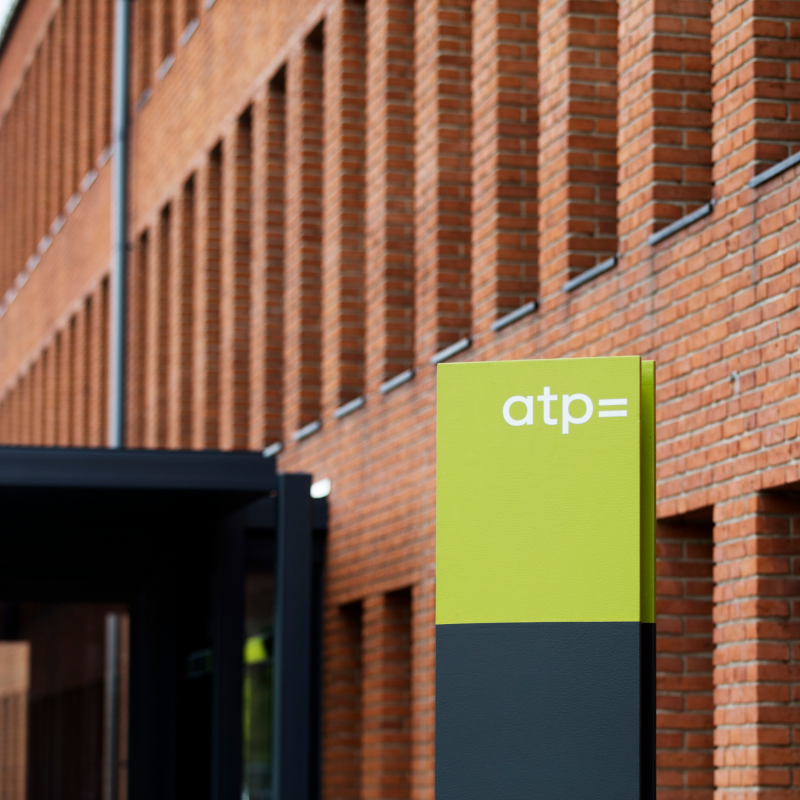
\includegraphics[width=0.75\textwidth]{atp-hq.png}
        \caption*{\textit{ATP headquarters at Hillerød\cite{about_atp}}}
\end{figure}

As the company operates in Denmark, I travelled there and resided near Hillerød with my relatives during the internship. My activities at ATP can be divided into two major parts: my experience with the Systems Architecture team and my work at the Help Desk, which will be detailed in the rest of this section. I was additonally given the opportunity to attend the Gartner Application Innovation \& Business Solutions summit. The following is a summary of the week of the internship by day, some of which was spent at home because of COVID-19 restrictions.

\begin{enumerate}
    \item First visit and tour of ATP headquarters, obtaining and understanding tools.
    \item Assisting meetings, briefing on systems architecture and working on system diagrams.
    \item (Remote) Attending the Gartner business summit.
    \item Making inventory of over 150 computers and monitors at Help Desk.
    \item Cancelled because of a COVID-19 outbreak, intended to be at Help Desk.
\end{enumerate}

Unfortunately, events on the fifth day were cancelled because of an outbreak of the COVID-19 Delta variant in Hillerød which prompted the closure of a school.\cite{covid_rip}. Indeed, a floorball\footnote[0]{A type of floor hockey with five players and a goalkeeper in each team} game with ATP workers (to which I invited) was scheduled to occur on that date at the school gymnasium.

\subsection{Systems Architecture}

On monday, I was given a company laptop and a set of over 20 "system diagrams" to analyse and work on. I learnt that Systems Architects create and make great use of these diagrams in order to visually break down a certain process into its component parts, and that they can be very diverse in scale and contents. They also serve to keep track of a system in its entirety and all its intricacies. 

\begin{figure}[H]
    \centering
        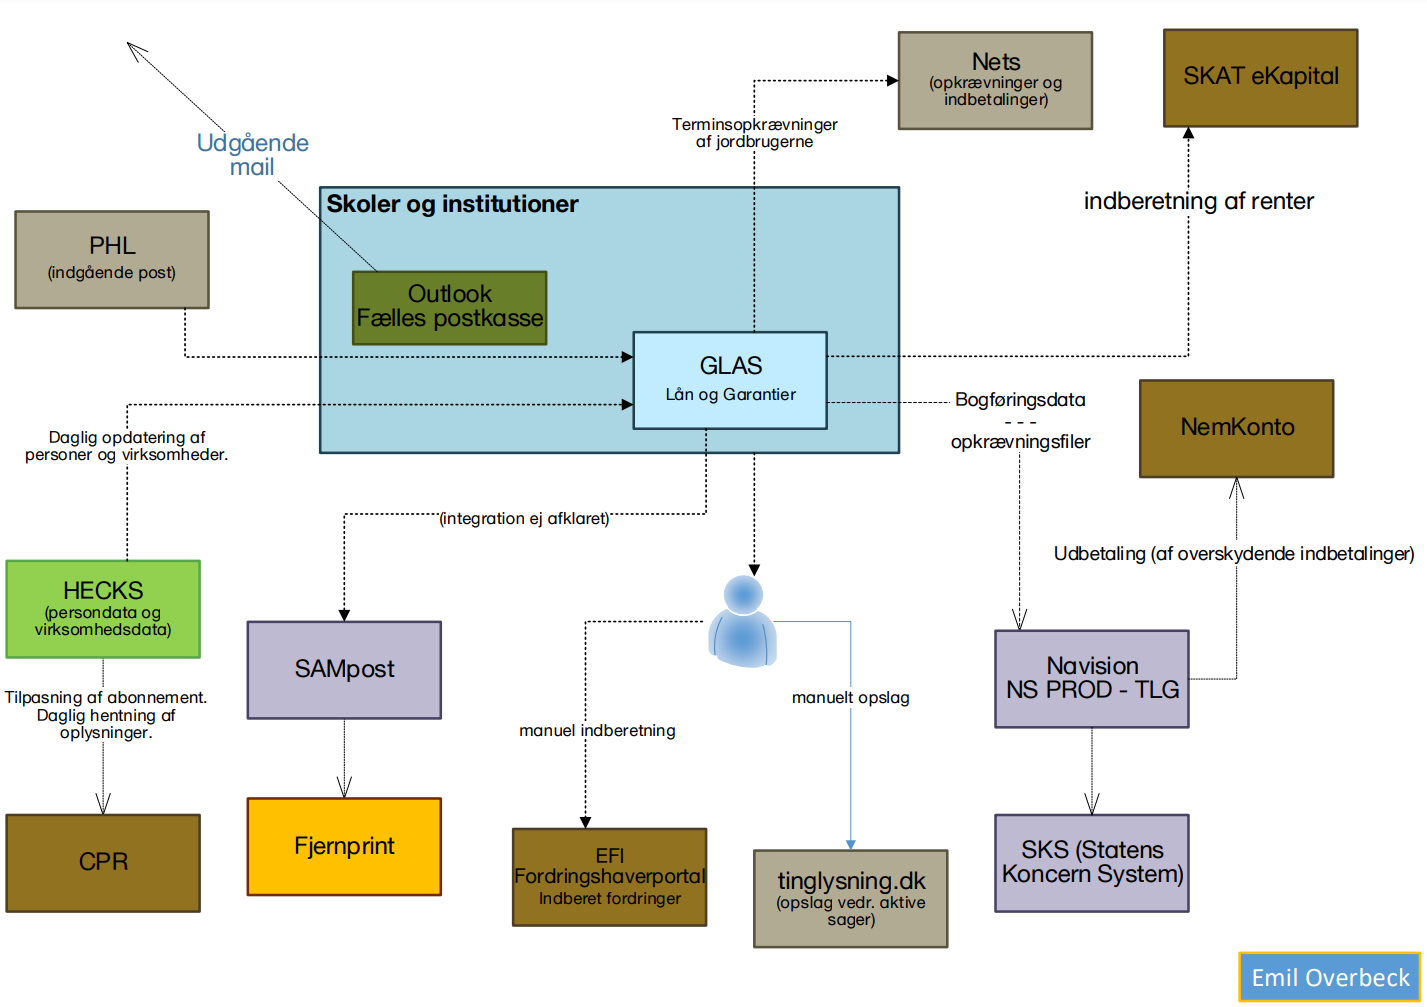
\includegraphics[width=1.00\textwidth]{image3.png}
        \caption*{\textit{Processing diagram for schools and instituions}}
\end{figure}

The above image is an example of one such diagram that I was instructed to complete while keeping it clear and consistent. It describes the financial processing service that ATP may provide to eduation institutions, which involves a multitude individual modules such as Microsoft Outlook and Skat eKapital, a financial reporting service. Moreover, it describes the interactions between these services. As an example, we can see that data must be manually registered to tinglysning.dk in order for that subsystem to function, as is meant by "manuelt opslag".

The following day, I was offered the opportunity to be individually briefed by a (french) member of the team. During this one hour session, I learnt several crucial elements concerning the profession, which have been summarised below.

\begin{itemize}
    \item At ATP, the systems architecture division consists of seven people, all of which originally worked as some form software engineer before being considered experienced enough to reach their current position. Thus, Systems Architecture requires techincal expertise and experience.
    \item Systems architects are also responsible for determining whether a certain technology is ready for use at the company without compromising security, efficiency or practicality. This has been especially important with the advent of the Cloud and the movement to outsource enterprise computing to it.
    \item Communication, as in explaining the nature and effects of projects to other departments, is one of the most important aspects of the profession. The reason for this is that plans for improving company systems may "never leave the drawing board" if said departments do not see its potential benefits.

    \begin{figure}[H]
        \centering
            
\includegraphics[width=0.50\textwidth]{triangle.png}
            \caption*{\textit{Systems Architecture triangle}}
    \end{figure}

    \item All systems are constrained by the elements above: Business, Economy and IT. I chose to present this relationship as a triangle because all of these concerns are interdependent. To illustrate, a new technology is only viable if it is useful to the business while remaining cost-effective and being practical to implement, so systems architects must take these elements into account and balance them according to the goals set by company leadership. 
    \item To plan for possible improvement, systems architects must document where and how various technologies are used. Systems used for HR, documentation, finance etc. may consist of technologies like, Oracle Java, SAP ERP, Ruby, SQL (for database management) and much more. Many of these may be in need of replacement or steamlining so as to benefit the Systems Architecture triangle previously mentioned.
\end{itemize}

% we need more info from later in the notes

\subsection{Gartner Summit}

The Gartner Application Innovation \& Business Solutions summit of 2021 is a series of presentations by industry experts intended to help business take full advantage of modern technologies and frameworks, like agile development and composable business architectures. This year's subject matter was "Building a Resilient Enterprise with Composable, Adaptable Applications". Thanks to ATP, I was able to attend four of these presentations, which have been summarised below.

\begin{enumerate}
    \item \color{dgreen} \textit{Delivering Resilience Through a Composability Fitness Routine}
    
    \color{black}COVID-19 proved that disruption can and will happen to all companies and illustrated that the most successful ones adapted to become more resilient and adaptable. But many were not as fortunate because they could not adapt based on rigid architectures, technologies and culture. This keynote discussed a composability fitness routine (an analogy to the human body) that can make any organization more resilient and fit for change, using elements like modularity, reusability, and autonomy.

    \item \color{dgreen} \textit{AI Engineering: How to Propel AI From Prototypes to Scalable Value Generators}
    
    \begin{figure}[H]
        \centering
            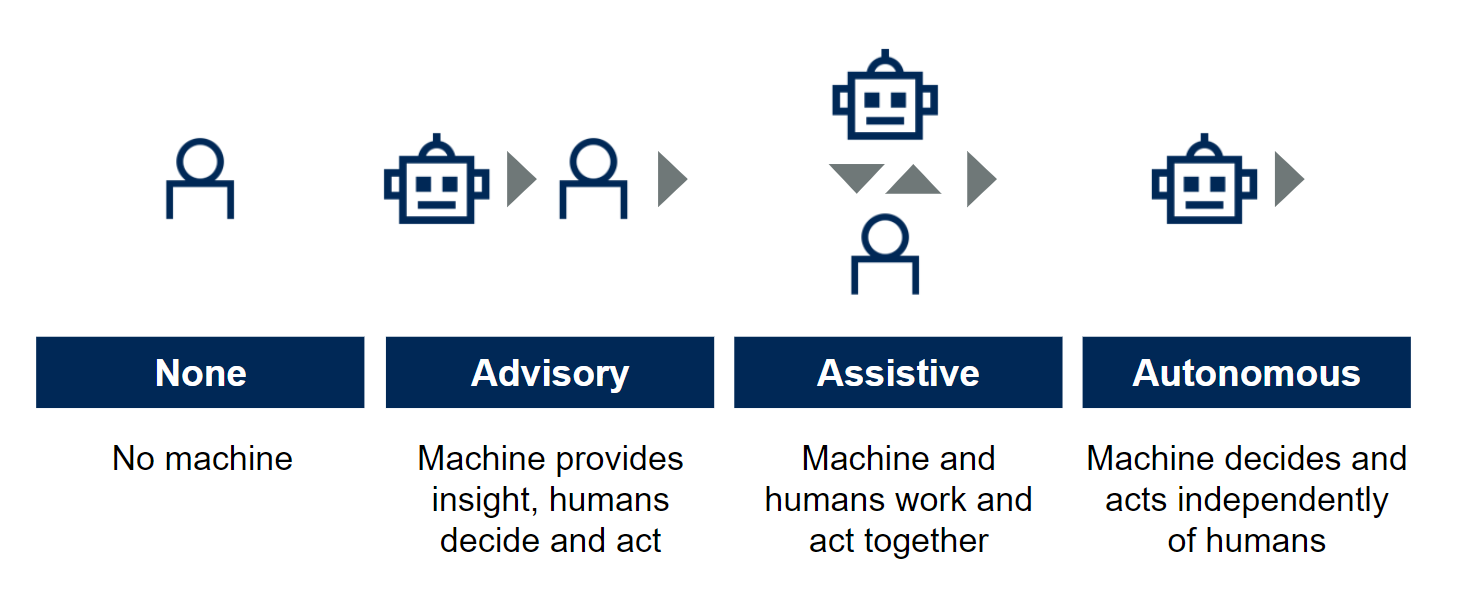
\includegraphics[width=1.00\textwidth]{image4.png}
            \caption*{\textit{Degrees of machine autonomy - Gartner}}
    \end{figure}

    \color{black} AI engineering brings together various disciplines from across organizations, while providing a path to generating value by deploying the combination of multiple AI techniques. AI engineering also includes responsible AI, dealing with risk, trust, transparency, ethics, fairness and accountability. An effective AI engineering practice will increase organizations’ ability to move AI projects beyond theory and into real-world applications. NASA is one such organisation: the Perseverance rover is an example of Generative AI, which can act  autonomously by determining its own instructions. Indeed, the communication delay between Earth and Mars is 50 minutes, rendering necessary a machine that can react to events without human intervention.

    \item \color{dgreen} \textit{Eggplant, part of Keysight Technologies: Modernizing an 80-Year-Old Tech Company}
    
    \color{black} Modernizing the application architecture of an 80-year-old multinational company is a daunting and complex task. Eggplant is ironically a tech company at the forefront of quantum computing and 6G Wireless, so speed was of utmost urgency. The host explained the importance of iteration and automation to transform the underlying application architecture and introduce new ways of working to strengthen the IT-Business relationship, like application diversification.

    \item \color{dgreen} Top 5 Priorities for Managing AI Risk Within Gartner’s MOST Framework
    
    \begin{figure}[H]
        \centering
            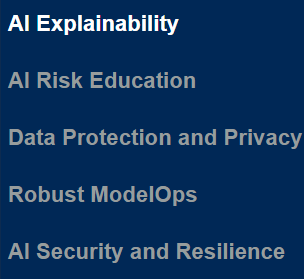
\includegraphics[width=0.50\textwidth]{image6.png}
            \caption*{\textit{The MOST framework - Gartner}}
    \end{figure}

    \color{black} The host presented Gartner's MOST framework for Managing AI Risk and a roadmap on the top five priorities within. The MOST covers model operations, security and trustworthiness for AI and adresses the following concerns: What are the various components of an AI risk management program? Who should manage our AI risk management program? What are the top five priorities for AI risk management and what existing tools can help us? In the example of BNP Paribas, a risk reporting and compliance team was formed to address the above concerns and mimise possible negative effects of AI technologies. In fact, by 2024, there will be twice the chance of negative outcomes for companies that don't have those security controls than for those that do. These consequences may include: hiring discrimination because of AI bias, susceptibility to data “poisoning” by bad actors, data and intellectual property theft through inference, and "Black box" scenarios where the actions of a model cannot be explained (e.g. why an interest rate is excessively high or why a loan got denied).

    \item \color{dgreen} API Security: How to Protect Your Organization From "Leaky APIs"

    \color{black} APIs are the ubiquitous protocols that allow different technologies to function and interface together. As such, they are required by everything from browsing the internet to enterprise datacentres. However, attacks and data breaches involving poorly secured APIs are increasing in frequency. API protection strategies include the use of API gateways, web application firewalls, access management, as well as specialist API security tools. As well as runtime protection, security should be applied to APIs at design time, including API security testing. This session covered API security best practices.
\end{enumerate}

\subsection{Hardware Inventory}

%\subsection{other}

\subsection{1+1}
